\chapter{INTRODUÇÃO}
\label{chp:intro}

Globalmente, gestores de todas as áreas de negócios enfrentam dificuldades para realizar a gestão das competências de seus colaboradores. Segundo \citeonline{Camargo2013}, com o início do século XXI, desafios alavancados por mudanças tecnológicas passaram a exigir dos profissionais novas aptidões.

De acordo com a \citeonline{CNI2013}, em indústrias pesquisadas no âmbito nacional, 65\% delas possuem dificuldades referente à falta de mão de obra qualificada, sendo que destas empresas, 90\% possuem dificuldade em encontrar operadores qualificados. Já no ano em 2014 a falta de mão de obra qualificada representou 13,2\% da frustração dos planos de investimentos das indústrias, sendo que em 2009 este percentual era de 8,8\% e, em 2012 apresentou seu maior pico 22,1\%.

Na empresa Franklin Electric (empresa do ramo metal mecânico, de Joinville-SC), estudo de caso desta pesquisa, existem funcionários com diferentes níveis de conhecimentos e competências, porém desconhecidas aos gestores e ao departamento de Recursos Humanos. Por intermédio desta realidade, torna-se difícil mensurar a existência de funcionários qualificados para ocupar cargos estratégicos na empresa. Outro problema que também preocupa os gestores é o fato de que muitas das competências na empresa Franklin Electric estão relacionadas ao conhecimento tácito destes indivíduos. Por exemplo, existem funcionários com uma vasta experiência profissional e que o nível de conhecimento técnico sobre os produtos da empresa Franklin Electric são expressivos, porem estão retidos somente a eles.

Por outro lado, segundo \citeonline{galvis2013critical} na última década, a Gestão do Conhecimento tornou-se um dos processos dentro da engenharia de software. Um número crescente de publicações trata este assunto a partir de diversas perspectivas, verificando-se o interesse predominante em temas como a codificação e o armazenamento, e a recuperação de conhecimentos utilizando tecnologias de informação. Temas como a criação, transferência e aplicação do conhecimento, no entanto, não foram tratados extensamente pela comunidade acadêmica. Além disso, os autores concluem que a maioria dos trabalhos de investigação empírica estão focadas na aplicação da Gestão do Conhecimento na melhoria de Processos de Software.

Deste modo, mapear, listar, classificar as competências dos funcionários e abstraí-las em um ambiente computacional, utilizando-se da união das gestões do conhecimento e por competências, motiva-se ao desenvolvimento de uma ferramenta, que auxiliara gestores na visualização das competências já existentes, ou de competências que necessitam ser alcançadas para o preenchimento de vagas com teor mais estratégico para a empresa.

\citeonline{Camargo2013} propôs um Plano de Desenvolvimento Organizacional a partir do mapeamento de competências dos trabalhadores das Unidades SESI/SENAI Curitiba e Região Metropolitana. Como resultado principal obteve-se maior comprometimento dos funcionários com a missão da instituição assim como por parte da empresa, que proporcionou abertura para que os colaboradores tenham autonomia na obtenção do conhecimento necessário para a sua função, refletido no planejamento de sua trajetória profissional.

Realizar o mapeamento das competências dos colaboradores na empresa Franklin Electric torna-se uma possível solução para suprir as necessidades óticas para obtenção ou retenção de talentos. Neste contexto, é possível obter uma solução computacional que supra as necessidades de gestão das competências dos colaboradores e que diminuam as lacunas entre as competências necessárias para uma função e as competências já obtidas pelos funcionários?

O objetivo geral desse trabalho é desenvolver um modelo para mapeamento de competências dos funcionários de uma indústria metal-mecânica. A fim de alcançar o objetivo proposto foi necessário realizar um estudo bibliográfico dos conceitos de Gestão por Competências e Gestão do Conhecimento, bem como desenvolver referências teóricas sobre o assunto em questão. Com estes dados apurados foi possível mapear as competências dos colaboradores da empresa Franklin Electric e definir métricas de cálculo para estas competências. Por fim desenvolveu-se um modelo para levantamento das competências e um modelo de ferramenta computacional capaz de realizar o trabalho de mensuração das competências.

A metodologia de pesquisa aplicada a este projeto é a exploratória, onde foi realizada uma pesquisa sobre o tema Gestão do Conhecimento, para buscar os mais variados conceitos, métodos e técnicas relativos ao problema definido para esta pesquisa. De acordo com os resultados obtidos no estudo bibliográfico, realizou-se um estudo de caso que apresenta o cenário industrial, sua localização, quantidade de funcionários, quantidade de departamentos. Neste cenário realizou-se uma delimitação para aplicação dos estudos e o caráter das informações colhidas será qualitativo.

A partir desta delimitação propõe-se um modelo de Gestão de Competências, com o auxílio de uma ferramenta computacional, propondo orientar gestores sobre decisões relacionadas as competências dos funcionários.

Esta pesquisa esta dividida em cinco capítulos sendo que o primeiro apresenta o objetivo geral e demais características sobre o trabalho. O segundo capitulo descreve o referencial teórico dos principais conceitos trabalhados nesta pesquisa. O capitulo três mostra o estudo de caso e desenvolvimento do modelo proposto. O quarto capitulo mostra a apresentação da empresa onde ocorreu a aplicação da proposta e apresenta os resultados obtidos. E, finalmente, o capitulo cinco apresenta a conclusão do trabalho bem como os trabalhos futuros.

\chapter{GESTÃO DO CONHECIMENTO E DE COMPETÊNCIAS}

O tema Gestão do conhecimento é definido por \citeonline{benfica2013proposta} como o gerenciamento dos intelectos presentes em uma organização. Sendo também visto como um conjunto de ações responsáveis por aumentar, de forma contínua, as competências dos funcionários e também a eficiências dos processos de negócios em uma organização, que contribui para o estimulo à aprendizagem.

A Gestão do Conhecimento é a união da “gestão”, que para \citeonline{rabaglio2012gestao} são os meios em que uma equipe, projeto ou instituição são administrados, e do “conhecimento” que para \citeonline{brandao2005gestao} liga-se ao “que” e “porque” fazer algo em determinado momento ou situação. Esta união, segundo \citeonline{Trainotti2014}, define-se como a identificação, criação, renovação e aplicação do conhecimento, estratégicos para a sobrevivência de uma organização.

Para \citeonline{gaspar2014gestao} a Gestão do Conhecimento é uma especialidade da área de Administração que consiste na aplicação de técnicas oriundas da Administração voltada ao conhecimento, com o objetivo de tornar estas técnicas, recursos a serem utilizados pelos colaboradores na execução de suas tarefas. Estas técnicas devem possuir condições de aplicar, disseminar, evoluir e atualizar o conhecimento no âmbito organizacional.

O conhecimento possui diferentes distinções e seu significado possui variação de pessoa para pessoa. Segundo \citeonline{Trainotti2014} o conhecimento está atrelado às crenças e culturas de uma pessoa sendo que o conhecimento pode ser adquirido por intermédio de duas vias: transferência de informações e de experiências de vida.

Quando transferido, o conhecimento pode ser analisado como uma combinação de três fatores: informação, contexto e experiência. O contexto pode ser definido à maneira do indivíduo enxergar a vida, ou seja, incluem-se influências como valores sociais, religião, cultural e gênero. Quando a informação é transmitido de uma pessoa para outra a qualidade da informação adquirida em forma de conhecimento fica sujeita ao contexto e à experiência do receptor \cite{SAJLIS1449}.

Para adquirir conhecimento, o ser humano pode optar por duas formas distintas, por meio do conhecimento explícito e ou pelo conhecimento tácito. O conhecimento de origem explicita é mais fácil para sere obtido, segundo \citeonline{Trainotti2014} o conhecimento explícito pode ser adquirido por intermédio de uma forma clara ou formulado em palavras. Este conhecimento pode ser obtido por exemplo, impressos em livros, revistas, artigos, apostilas e em expressões matemáticas.

Outro método para obtenção do conhecimento é o tácito, este por sua vez é mais difícil de ser trabalhado, pois é um conhecimento individual pertencente somente a uma determinada pessoa. Para \citeonline{camara2012gestao} o conhecimento tácito está atrelado ao indivíduo que o possui, é intransferível, foi adquirido ao longo da vida. Este tipo de conhecimento pode ser observado na forma de conceito, expressões, ideias em e-mails, reuniões, telefonemas, mais relacionado a experiência das pessoas.

Para \citeonline{Trainotti2014} com o passar dos anos as organizações perceberam que o ativo essencial para manter a competitividade e as estratégias de seus negócios são as pessoas, pois são elas que possuem o conhecimento sobre seus procedimentos e processos. Na indústria o conhecimento tácito promove preocupações aos gestores, isto porque este tipo de conhecimento, segundo \citeonline{rabaglio2012gestao}, caracteriza-se por ficar retido ao funcionário que realiza uma determinada tarefa sendo que nenhum outro executaria da mesma forma.

\citeonline{pitrowsky2014organizational} argumenta que a importância da dimensão do conhecimento tácito não mostra nenhum entendimento da organização como uma máquina de processamento de informações, mas sim como um organismo vivo com uma cultura que reconheça que nem todo conhecimento é criado e aprendido em uma forma puramente consciente. Uma vez que é o resultado da interiorização das experiências vividas por indivíduos, ou seja, nem sempre é possível transmitir conhecimento somente por intermédio de educação formal e treinamentos.

Segundo \citeonline{Trainotti2014} a realização da divisão do conhecimento de cada indivíduo e o compartilhamento destes de uma forma coerente para uma organização é o grande desafio para as empresas. Uma das maneiras para esta divisão é a conversão do conhecimento tácito para o explícito sendo que esta transformação é a principal maneira para a criação do conhecimento organizacional.

A gestão do conhecimento possui diversas elucidações, porém \citeonline{benfica2013proposta} aborda que muitas das definições de gestão do conhecimento acabam não englobando os aspectos relacionados à sistematização do conhecimento que envolve a área de TI como apoiadora deste processo. Logo, o conceito de gestão do conhecimento definido por Benfica e Faria (2013) caracteriza-se como um conjunto de atividades que funcionam de acordo com a geração, codificação e transferência do conhecimento.

Para que toda a sistematização da gestão do conhecimento ocorra é necessário que haja uma cultura de disseminação do conhecimento em uma organização, onde \citeonline{Trainotti2014} afirma que a disseminação de informações entre os colaboradores contribui ao gerenciamento do conhecimento organizacional que se reflete no oferecimento de diferencias aos clientes. Porém existe uma dificuldade na retenção destes conhecimentos.

Para realizar a gestão do conhecimento em uma organização existe a premissa relacionando os colaboradores para que possam ser estimulados pelos seus gestores a se expressarem livremente. Como contribuição a esta premissa foram criados modelos que servem de auxílio as empresas e contribui a sua eficiência por meio do estudo detalhado ao comportamento e estrutura corporativa. Neste contexto a computação serve para auxiliar a estes modelos, e cria artefatos para a disseminação do conhecimento \cite{Trainotti2014}.

Para \citeonline{benfica2013proposta} as ferramentas de gestão do conhecimento servem para identificar, estruturar e tornar disponível o conhecimento. O objetivo principal desta gestão é a modelagem do conhecimento retida na cabeça dos funcionários ou em documentos corporativos e por sua vez disponibilizada para toda a organização.

Segundo \citeonline{camara2012gestao} as construções de artefatos computacionais tomam base não somente a gestão do conhecimento, também necessita haver contribuição por parte da gestão por competências. A utilização destas duas gestões justifica-se pelo fato de que trabalhadores mal remunerados ou desqualificados tecnicamente realizam serviços com baixa qualidade, desta forma isto afirma a necessidade da utilização da gestão por competência como alternativa a estes problemas. Já a gestão do conhecimento serve para proteger e disseminar o conhecimento e as práticas.

Em análise a teoria da Gestão do conhecimento fica evidenciado a importância da construção de um modelo de mapeamento de competências, a fim de suprir a necessidade de conhecer não somente a lacuna, mas também a obtenção das qualificações que um individuo possui em uma determinada área de atuação.

A gestão por competências segundo \citeonline{brandao2005gestao} consiste no planejamento, captação, desenvolvimento e avaliação referente aos diferentes níveis organizacionais (individual, grupal e organizacional), sempre com o foco nas competências necessárias para atingir os objetivos de uma organização. Trata-se de um processo continuo que se inicia com a formulação das estratégias organizacional como missão, visão e objetivos, logo após são definidos os indicadores de desempenho e metas baseadas nos objetivos estratégicos.

\citeonline{Camargo2013} retrata a gestão por competências como um processo contínuo com base nas estratégias organizacionais, uma das etapas é a identificação das competências necessárias que atinjam o desempenho esperado. Este modelo de gestão concentra-se no planejamento, captação, desenvolvimento e avaliação nos diferentes níveis de uma organização para obtenção das competências necessárias para alcançar os objetivos.

O conceito de competência segundo \citeonline{bomfim2012competencia} surgiu por meio da necessidade de uma abordagem que possuísse maior efeito referente à escolha de pessoas para as organizações. A abordagem anteriormente utilizada, o teste de inteligência, não possuía referência para a compreensão e a construção de ferramentas da gestão de pessoas.

Para \citeonline{oliveira2014percepccao} a competência possui maior significância do que um conhecimento ou uma habilidade. A competência de um indivíduo é uma característica individual que se adquire devido as suas experiências profissionais, seu empenho caracterizado no querer aprender, sua busca por conhecimento ou também por estar envolvido dentro de um determinado contexto profissional.

De acordo com \citeonline{lang2014aprendizagem} para o correto entendimento de competência é necessário à distinção de competência e habilidade. O significado de habilidade refere-se à capacidade de executar tarefas com exatidão e facilidade e também se adaptar a mudanças. Já a competência trata-se de um sistema complexo que aborda habilidades intelectuais, habilidades que envolvam atitudes e também outras não cognitivas.

Segundo \citeonline{oliveira2014percepccao} a competência em um indivíduo manifesta-se na forma como ele enfrenta as situações anormais a sua função, por intermédio de sua inciativa e até mesmo de seu improviso em situações que fogem a programação atual. Este comportamento torna-se cada vez mais importante pois a competência profissional não pode mais ficar atrelada apenas a tarefas pré-definidas.

A seguir será apresentado a evolução do conceito competência com o intuito de se obter o quanto esta gestão foi aperfeiçoada durante o tempo e se existem motivadores para a gestão por competências continuar a sua evolução.

\section{EVOLUÇÃO DO CONCEITO COMPETÊNCIA}

A evolução do conceito competência manifesta-se por meio da percepção de que não basta apenas “saber por saber”, mas sim o “saber para fazer”, por esta razão fica claro o motivo de realizar determinadas tarefas e também esclarece a razão de que para a realização de determinada tarefa exista várias maneiras de serem executadas \cite{schlatter2014administrador}.

\citeonline{schlatter2014administrador} aborda que, devido às exigências, o conceito de competência passou a ser abordado como um conjunto de recursos, estes constituídos por conhecimentos, habilidades e atitudes que informalmente foi denominado CHA. No Brasil o CHA é o conceito mais difundido entre os profissionais de RH podendo também citar a França como grande utilizadora.

O CHA iniciou-se na década de 70 e era conhecido como CH, pois nesta época eram valorizadas apenas as competências técnicas (conhecimento e habilidade). Desta forma as ações referentes a um empregado (demissão, admissão, promoção) em uma organização eram feitas apenas com base nas competências técnicas, por onde as empresas obtiveram grandes prejuízos \cite{rabaglio2012gestao}.

Atualmente o CHA é amplamente utilizado na sua forma completa “C” “H” “A”, para um melhor entendimento de cada um dos componentes, pode-se visualizar na tabela 1 que apresenta maiores detalhes de cada componente.


\begin{table}[htbp]
	\centering
	\caption{Componentes do CHA}
	\label{tab:exTabela}
	\begin{tabular}{l|l}

		\hline
		& \textbf{Para o cargo:} refere-se à necessidade que o cargo tem de\\
		& formação acadêmica, conhecimentos técnicos, especialidades.\\
		& Nessa etapa da competência, não se exige prática, apenas \\
		Conhecimento     & formação e pré-requisitos necessários ao cargo.\\
		& \textbf{Para o candidato:} refere-se à especialidade de sua formação,\\
		& escolaridade, idiomas, informática, para atender as necessidades \\
		& do cargo etc. \\
		\hline
		& Experiência, prática, domínio do conhecimento.\\
		& Esse termo é muito usado no esporte quando se refere aos atletas\\
		Habilidades & com prática e domínio naquilo que realizam. Alguns cargos   \\
		& precisam de muita experiência nas atribuições, portanto, precisam \\
		& de Habilidade.\\
		\hline
		& Valores, emoções, sentimentos expressos por meio do\\
		& comportamento humano, que, por meio de uma metodologia, \\
		Atitudes    & tornam possível identificar o perfil comportamental necessário para    \\
		& cada cargo. \\
		\hline

		\end{tabular}\\
	\vspace{2mm}
 \footnotesize Fonte: o autor
\end{table}

De acordo com \citeonline{Camargo2013} o CHA pode ser entendido como as dimensões, conhecimento este que diz respeito a informações assimiladas e estruturadas pelo indivíduo que o faz entender o mundo. O universo da habilidade, possui ligação ao saber fazer. Utilizar o conhecimento adquirido de forma produtiva com o objetivo de atingir um propósito.

Abaixo são apresentados modelos de gestão por competências baseados no conjunto CHA que \citeonline{Camargo2013} representou em sua monografia:

\begin{alineas}
	\item Modelo Iceberg \citeonline{spencer1993competence} – Neste modelo (Figura 1) a autora aborda a visualização das competências em dois níveis, um nível onde estão as competências no modelo CH, estes fácil de serem identificados e em um nível não visível estão as competências relacionadas a personalidade de cada indivíduo. Neste modelo fica evidente a não abordagem do componente Atitude.;

	\begin{figure}[htbp]
		\centering
		\caption{Modelo Iceberg por Spencer e Spencer}
		\includegraphics[width=1.0\textwidth]{figuras/iceberg.png}

		\label{fig:ICEBERG}
		\footnotesize Fonte: Baseado em \citeonline{spencer1993competence}
	\end{figure}
	 \vspace{5mm}

Este modelo mostra como o comportamento de um individuo pode ser comparado a um iceberg. Conhecimento e habilidades tendem a ser mais visíveis, em quanto o autoconceito, recursos e motivação ficam mais ocultos, profundos ou centrais na personalidade de um individuo. Olhando de cima, apenas parte das habilidades podem ser vistas, sendo que a parte visível, é apenas reflexo da oculta \cite{Molina2010}.

	\item Árvore de Competência \citeonline{gramigna2002modelo} – Este modelo (Figura 2) engloba os três componentes do CHA desta forma os galhos representam as habilidades, o tronco representa o conhecimento e a raiz representa as atitudes. As três dimensões podem ser analisadas no seguinte contexto: o que precisa ser feito (conhecimento), como deve ser feito (habilidades) e porque será feito (atitudes).

	\vspace{30mm}

	\begin{figure}[htbp]
		\centering
		\caption{Árvore de Competência por Gramigna}
		\includegraphics[width=0.55\textwidth]{figuras/arvore.png}

		\label{fig:ARVORE}
		\footnotesize Fonte: Baseado em \citeonline{gramigna2002modelo}
	\end{figure}

Segundo \citeonline{Masih2008gestao} a árvore das competências é uma modelo que possui maior difusão em relação ao modelo Iceberg. A árvore das competências possui sua base no conceito CHA e de forma mais simples comparado ao modelo Iceberg mostra a estruturação das competências por meio da combinação do conhecimento, habilidade e atitude. O modelo em questão da mesma maneira que o modelo Iceberg não relaciona os elementos  competência, comportamento e desempenho.

	\item	Casa das Competências \citeonline{ruzzarin2002gestao} – Neste modelo (Figura 3) as competências dos indivíduos são verificadas como competências técnicas (conhecimento) e competências comportamentais (habilidades e atitudes) de cada função, sendo que o telhado (responsabilidades) possui a descrição do que se espera para o cargo. Os pilares representam as competências e a base representa os esforços de treinamento e desenvolvimento.
	\vspace{30mm}

	\begin{figure}[htbp]
		\centering
		\caption{Casa das competências}
		\includegraphics[width=0.8\textwidth]{figuras/casa.png}

		\label{fig:CASA}
		\footnotesize Fonte: Baseado em \citeonline{ruzzarin2002gestao}
	\end{figure}

\end{alineas}

A casa das competências em relação aos modelo Iceberg e Árvore do conhecimento, realiza o agrupamento das competências técnicas e comportamentais, considerando os resultados esperados, e vincula a estrutura das competências com um plano de desenvolvimento. Este modelo como destaque mostra os resultados esperados para o cargo (Responsabilidades) sendo que este aspecto é o que mais ocasiona criticas ao conceito CHA \cite{Masih2008gestao}.

	Segundo \citeonline{schlatter2014administrador} a maioria dos conceitos abordados focam no indivíduo e na maneira como ele utiliza o CHA para realizar uma tarefa com facilidade. Porém existem tarefas que necessitam do trabalho coletivo para serem realizadas, logo a distinção de competências individuais e competências organizacionais se fazem necessárias assim como a descrição onde as duas se complementam.

	Para \citeonline{oliveira2014percepccao}, por intermédio dos novos modelos de gestão, é notável a ênfase dedicado as pessoas como principal recurso em uma organização. A competitividade proporciona a busca por profissionais capacitados para execução de tarefas. Somente por meio desta premissa a gestão por competência torna-se instrumento diferencial de mercado, porem se faz necessário o envolvimento dos diversos níveis da organização.

\section{COMPETÊNCIAS INDIVIDUAIS}

As competências individuais possuem sua formação na qualificação e no mapeamento das funções. Neste sentido, as qualificações estão ligadas aos requisitos do cargo que o indivíduo possui ou também por intermédio do conhecimento que o indivíduo adquiriu ao longo do tempo. Também se pode afirmar que parte deste conhecimento foram adquiridas no sistema educacional \cite{oliveira2014percepccao}.

As competências individuais podem ser definidas segundo \citeonline{almeida2015certificaccao} como o saber agir responsável e reconhecido, onde que este agir responsável e reconhecido implica na agregação de valor econômico a empresa e também no valor social ao indivíduo. A pessoa competente é aquela que enfrenta frequentemente situações fora de sua rotina normal, situações imprevistas e variáveis que deste modo contribuem para a sua evolução \cite{Bergamini2012}.

Na figura 4, ficam claras as necessidades de um indivíduo referente a extração dos insumos necessários para obtenção de um desempenho aceitável. Estas ligações resultam na retenção de Valores Econômicos a empresa e a Valores sociais ao indivíduo \cite{almeida2015certificaccao}.

\begin{figure}[htbp]
	\centering
	\caption{Fonte de Valores das Competências}
	\includegraphics[width=1.0\textwidth]{figuras/fvc.png}

	\label{fig:FVC}
	\footnotesize Fonte: Adaptado \citeonline{almeida2015certificaccao}
\end{figure}

Para \citeonline{fariacosta2014} as competências possuem variação de acordo com o contexto do indivíduo no momento, desta forma o que dá sentido à competência é a interação com o meio que ocorre via gestão de competências. Na tabela 2 estão descritas as principais competências possíveis de um indivíduo.
\vspace{30mm}

\begin{table}[htbp]
	\centering
	\caption{Competências para o Profissional}
	\label{tab:competencia_profissional}
	\begin{tabular}{l|l} \hline

		\hline
		Saber Agir & Saber o que e por que faz. Saber julgar, escolher, decidir.\\
		\hline
		Saber mobilizar & Criar sinergia e mobilizar recursos e competências. \\ Recursos& \\
		\hline
		Saber comunicar & Compreender, trabalhar, transmitir informações, conhecimentos. \\
		\hline
		Saber aprender     & Trabalhar o conhecimento e a experiência, rever modelos mentais;\\
		&  saber desenvolver-se.\\
		\hline
		Saber engajar-se  & Saber empreender, assumir riscos. Comprometer-se.\\
		e comprometer-se &  \\
		\hline
		Saber assumir  & Ser responsável, assumir os riscos e consequências de suas ações \\
		responsabilidades & e ser por isso reconhecido. \\
		\hline
		Ter visão estratégica & Conhecer e entender o negócio da organização, o seu ambiente, \\
		& identificar oportunidades e alternativas.

		\\
		\hline
	\end{tabular}
	\vspace{2mm}
	\\ \footnotesize Fonte: \citeonline{fariacosta2014}
\end{table}

\citeonline{lang2014aprendizagem} aborda um conceito de competência baseado no agir de forma autônoma, agir de acordo com cada situação. Este conceito caracteriza-se pela capacitação de indivíduos referente ao seu desenvolvimento e também de incentivos para se expressarem livremente. Este tipo de conceito necessita de orientações para o futuro, permitindo que o indivíduo tenha consciência do seu ambiente e sua participação.

Para \citeonline{dutra2004competencias}, um profissional deve se entregar a uma organização de forma efetiva, porém o objetivo, tanto do profissional quanto da organização deve ser o mesmo para que o excesso de entrega não possa interferir no desempenho. A discussão sobre o conceito de entrega é de grande valia para ficar bem definido o doar-se a organização e o saber agir responsável. Muitas empresas valorizam os profissionais por seus atos dentro da organização, e deixa de lado a descrição formal de suas funções e atribuições.

De acordo com \citeonline{oliveira2014percepccao} as competências individuais não ficam limitadas apenas ao conhecimento tácito adquiro ao decorrer da sua vida, e também não somente estão ligados a tarefa que o indivíduo realiza. O conhecimento e o \textit{know-how} apenas adquirem o status de competência por intermédio da comunicação ou troca deste conhecimento, o que torna-se assim de suma importância a rede de conhecimento na qual está inserido, para que a competência se torne aplicável.

Após ser explicado o conceito de competência individual serão conceituadas as competências organizacionais importantes para a construção do mapeamento das competências.



\section{COMPETÊNCIAS ORGANIZACIONAIS}

Competência Organizacional é o resultado da integração dos recursos, habilidades e processos organizacionais. Tal competências são responsáveis pela geração de vantagens competitivas de uma empresa. As competências organizacionais necessitam ser desdobradas em individuais para que não ocorra o pensamento de preenchimento de cargo, mas sim o preenchimento de competências que a tornem inovadora e competitiva \cite{freitas2014proposta}.

Porém de acordo com \citeonline{oliveira2014percepccao} as competências essenciais, que são formadas por um conjunto de habilidades responsáveis por permitir a uma empresa entregar benefícios aos seus clientes, necessita estar em constante adaptação. Isto porque somente elas não são suficientes por manter uma empresa em uma posição competitiva no mercado.

\citeonline{pereira2011competencias} afirma que as competências organizacionais devem convergir rumo ao planejamento estratégico da empresa assim como a sua cultura, e que estes estarão em constante mudanças e isto exigi adaptações com o foco na vantagem competitiva. Para se manterem ativas, as organizações necessitam buscar excelência nas gestões de negócios e processos para que a criticidade se converta em benefícios a organização, seus funcionários e seus clientes.

\citeonline{bomfim2012competencia} diferencia as competências organizacionais das essenciais sendo que as competências organizacionais são as necessárias para o desenvolvimento das atividades referente a cada função. Já as competências essenciais são aquelas que seguem um determinado critério como: oferecem reais benefícios aos clientes; são difíceis de copiar e dão acesso a diferentes mercados.

As competências que são essenciais a uma empresa estão diretamente ligadas a estratégia empresarial assim como o capital de conhecimento desta empresa. Por meio disto acredita-se que o mapeamento destas competências individuais da empresa garanta sua sobrevivência \cite{oliveira2014percepccao}.

Para \citeonline{freitas2014proposta} as competências essenciais necessitam ser convertidas em competências funcionais únicas para cada área ou unidade da empresa. As competências funcionais também devem ser convertidas, essa conversão deve ocorrer de funcionais para individuais pelo motivo de que não se trata apenas de preenchimento de cargos, mas sim é necessário possuir competências que resultem em inovação e competitividade.

Para ser corretamente entendido os conceitos de competências individuais e competências organizacionais, a seguir será explanado onde começa e onde termina as competências organizacionais e individuais.

\section{DA COMPETÊNCIA INDIVIDUAL A COMPETÊNCIA ORGANIZACIONAL}

A competência é o resultante da interação e complemento de habilidades e conhecimentos individuais e de grupos de uma organização. As competências organizacionais são mais do que um conjunto de competências individuais, elas potencializam recursos, capacidade e qualificações no que resulta em uma competência coletiva responsável por conduzir e orientar a organização em suas estratégias \cite{almeida2015certificaccao}.

De acordo com \citeonline{schlatter2014administrador} no momento que se verifica o aumento da complexidade dos serviços que se fazem necessários a ser entregues a sociedade, apenas o conceito de competência individual não é o suficiente. A partir deste cenário ocorre a necessidade de competências coletivas, ou seja, a interação entre as competências individuais de um determinado grupo.

Para \citeonline{zago2013cultura} uma das mais importantes fundamentações é a construção da relação entre empresas e comportamento de indivíduos. Existe uma interação muito grande entre essas duas partes, de forma que cada parte constitui a outra. Desta forma uma empresa é reflexo de seus funcionários e grupos de funcionários, quando os funcionários agem conforme uma convenção social suas ações caracterizam-se conforme a convenção na qual ela pertence.

Segundo \citeonline{Camargo2013} um diagnóstico resumido sobre as competências essenciais pode ser realizado em duas etapas. Como primeira etapa analisa-se as competências empresariais, ou seja, as já instaladas e a competências a serem adquiridas de modo que a torne cada vez mais competitiva. A segunda etapa realiza uma avalição nas competências humanas, as que precisão ser adquiridas e também as que necessitam ser desenvolvidas, isto para que a empresa tenha sucesso em seus objetivos estratégicos.

As competências individuais e coletivas se modelam e se estruturam conforme as competências organizacionais de uma empresa, conforme representado na Figura 5. Deste modo as pessoas e as organizações lado a lado realizam um processo continuo de troca de competências e formam os diferentes níveis de agregação de competências (individual, coletiva e ambiental) \cite{zago2013cultura}.

\begin{figure}[htbp]
	\centering
	\label{fig:modelo_por_competencia}
	\caption{Formação do modelo de Gestão por Competência}
	\centering
	\includegraphics[width=1.0\textwidth]{figuras/fmgc.png}

	\footnotesize Fonte: Baseado em \citeonline{zago2013cultura}
\end{figure}

Esta seção apresenta a importância das competências tanto organizacional como individual e valida o quanto estes dois conceitos juntos são essenciais para a construção de artefatos como o mapeamento de competências. A seguir será apresentado a diferença da antiga maneira de gerir pessoas em relação a gestão por competências.


\section{GESTÃO DE PESSOAS POR COMPETÊNCIAS VERSUS GESTÃO TRADICIONAL DE PESSOAS}

Segundo \citeonline{amaral2008gestao} a forma de realizar a gestão de pessoas nas empresas no decorrer dos últimos anos criou um grande desconforto tanto para o funcionário quanto para os gestores e profissionais de RH. Isto implica em uma grande irregularidade em relação à forma tradicional de gestão e as necessidades das empresas modernas e também as necessidades dos funcionários.

\citeonline{dos2012gestao} afirmam que desde a década de 80, a gestão tradicional de pessoas era questionada, isto porque os ambientes organizacionais estão em constante mudanças, o que passou a exigir novas formas de gestão. Esta realidade ocorre devido à abertura de mercado e também devido a globalização que intensifica o uso de tecnologia, não somente nos processos produtivos, mas também nas áreas administrativas e de logística.

\citeonline{hondeghem2014modelos} abordam que o inicio da noção de gestão por competência ocorrem nos EUA e Reino Unido justamente no ano de 1980 quando nesta época foi tentado primeiramente o aumento do nível de desempenho educacional pelo motivo que eles eram os responsáveis por não atender as demandadas do mercado de trabalho. Por segundo, foi atentado para a força de trabalho e a falta de mão de obra qualificada nas indústrias. Isto fez o Reino Unido criar um sistema conduzido pelas próprias indústrias, este sistema consistia no estabelecimento de critérios de desempenho para todos os setores industriais.

No Brasil, a gestão por competências ganhou força a partir do ano de 2000 sendo assim ainda é um conceito novo, porém as contribuições relacionadas a esta gestão são as mais recentes e conquistou espaço nas revistas de publicações cientificas mais renomadas. O modelo Brasileiro por ser jovem, ainda requer maiores esclarecimentos, disseminação e aprofundamento \cite{zago2013cultura}.

Para \citeonline{publica2012analise} a Gestão por Competências se consolida como uma alternativa para a Gestão tradicional de pessoas. Com base na informação de que o domínio de alguns recursos é resultante do desempenho da organização, a Gestão por Competências possui a proposta de integrar e direcionar esforços focados na gestão de pessoas, com a visão do desenvolvimento e sustentação dos valores considerados fundamentais para a obtenção do objetivo e da missão organizacional.

O conhecimento é o ativo com maior importância em uma empresa, por esta razão os processos que permeiam o conhecimento passam a ser importante desde sua produção até sua disseminação. Neste contexto gerenciar o conhecimento que se possui torna-se indispensável a uma organização e gestões como a de competências torna-se um importante modelo ainda mais com a utilização de ferramentas como o mapeamento de competências \cite{torres2012mapeamento}.

A seguir será abordado o que é o mapeamento de competências, assim como a sua importância para com a gestão das competências de funcionários em uma organização.

\section{MAPEAMENTO DAS COMPETÊNCIAS}

Segundo \citeonline{freitas2014proposta} o modo como as empresas gerenciam seus funcionários está em processo de mudança isto porque os tipos de gestão, como a de competências, tornam-se cada vez mais obrigatório para manter o nível de competitividade entre as empresas. É necessário administrar com as pessoas ao invés de administrar as pessoas, desta forma é possível manter um funcionário motivado, o que o torna mais competitivo.

De acordo com \citeonline{torres2012mapeamento} o mapeamento das competências permite identificar, sistematizar e evidenciar as competências em uma empresa, isto torna fácil à localização e identificação das lacunas de conhecimento. Este mapeamento possibilita o correto direcionamento de funcionários ou até mesmo justifica a contratação de novos para áreas mais fracas de conhecimento. Outro benefício se dá por meio da identificação da necessidade de qualificação dos funcionários.

\citeonline{Camargo2013} afirma que o mapeamento das competências visa identificar as lacunas de conhecimento (\textit{gaps}), ou seja, visa identificar as diferenças entre as competências necessárias e as competências internas já existentes. O não tratamento desta diferença (\textit{gap}) tornará a empresa, ao decorrer dos anos, defasada e implica assim na falta de competitividade e no aumento do investimento para redução da lacuna.

O mapeamento das competências possui o objetivo de identificar e tornar operacional as competências individuais existentes em uma organização. Este mapeamento é realizado por meio da observação no local de trabalho que consiste em procurar as lacunas de competências para o desenvolvimento da captação de profissionais. Após a conclusão do mapeamento e da identificação das competências é recomendado à definição de um perfil, este baseado no CHA \cite{publica2012analise}.

Para \citeonline{amaral2008gestao} o mapeamento das competências consiste no esclarecimento das competências da organização e dos funcionários com base nos indicadores destas competências. Os indicadores consistem nas informações referente a cada cargo que, este conhecimento pode se dar por meio de vários mecanismos por exemplo: Observação da atuação do profissional, análise da descrição de cargo, etc.

O mapeamento de competências para \citeonline{publica2012analise} além de servir como base nos processos de recrutamento e treinamento, também serve para auxilio referente ao acompanhamento e avaliação de resultados na forma de \textit{feedbacks} para a organização afim de indicar possíveis desvios na execução de planos e indicadores de desempenho.
\vspace{30mm}

\citeonline{rabaglio2012gestao} lista cinco passos para a realização do mapeamento das competências. Estes passos podem ser visualizados na Quadro 1.


\begin{quadro}[htbp]
	\centering
	\caption{Passos para o Mapeamento das Competências}
	\label{tab:passo_mapeamento}
	\begin{tabular}{|l|l|} \hline

		\hline
		PASSO & DESCRIÇÃO\\
		\hline
		1º Encontrar os indicadores de  & Identificação dos indicadores na descrição de \\
		competências do cargo. & cargos e funções. Indicadores são atribuições ou \\
		& atividades do cargo. \\
		\hline
		2º Extrair as competências técnicas e  & Análise de cada um dos indicadores para extrair \\
		comportamentais dos indicadores de & as competências técnicas e comportamentais \\
		competências do cargo. & necessárias para a excelência na realização do \\
		& indicador.\\
		\hline
		& Competências técnicas são pré-requisitos para o  \\
		3º a) Relacionar as competências & cargo, estas competências são aferidas por meio \\ técnicas.
		& de teste, construídos e corrigidos pela própria \\
		& área solicitante em parceria como RH.\\
		\hline
		& Nenhum comportamento é exibido isoladamente;\\
		3º b) Organizar as competências & Sempre que um comportamento é exibido, leva \\
		comportamentais em grupos de & com ele uma quantidade de outros \\
		competências similares. & comportamentos similares ou que sejam \\
		& requisito para aquele comportamento.\\
		\hline
		& Relacionar possíveis nomes de grupos de \\
		3º c) Nomear os grupos de &  competência similares, a base para criação  \\ competências.
		& desses grupos são a descrição e atribuição dos  \\
		& cargos ou funções. \\
		\hline
		4º Justificar a necessidade de cada & A justificativa é uma explicação sobre o uso das \\
		grupo de competências similares & competências nas atribuições de cargos, sempre \\  para o cargo.
		& na forma situacional.\\
		\hline
		& A base da mensuração das competências  \\
		5º Mensurar as competências.   & também são os indicadores de competências.  \\
		& Para esta etapa é importante a utilização de um \\
		& software dinâmico.

		\\
		\hline
	\end{tabular}
	\vspace{2mm}
	\\ \footnotesize Fonte: \citeonline{rabaglio2012gestao}
\end{quadro}


Para \citeonline{rabaglio2012gestao} o fator chave para o mapeamento da competências é a descrição de cargos ou a descrição das funções. Este fator chave fornecerá todos os indicadores de desempenho do cargo sendo que será a base para a mensuração das competências.

No fluxograma da Figura 6, pode-se visualizar o processo para o mapeamento das competências em uma organização.

\begin{figure}[htbp]
	\centering
	\label{fig:fluxo_mapeamento}
	\caption{Fluxo do processo de Mapeamento}
	\centering
	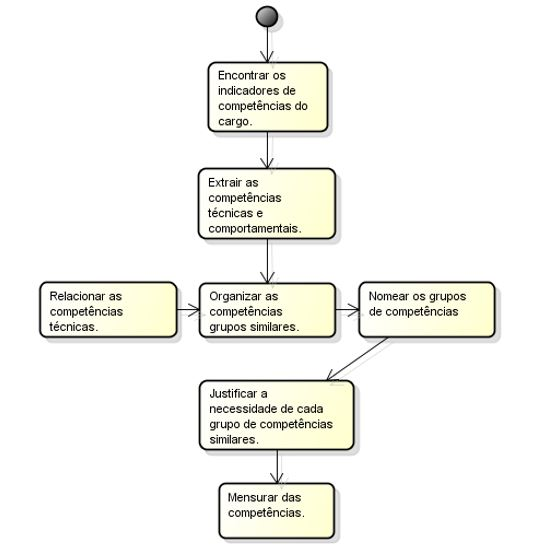
\includegraphics[width=1.0\textwidth]{figuras/fluxo_mapeamento.jpg}

	\footnotesize Fonte: Baseado em \citeonline{rabaglio2012gestao}
\end{figure}

Segundo \citeonline{gramigna2007competencias} atualmente vivemos algo inusitado, pois no momento em que as organizações achavam que possuíam talentos de sobra, na verdade se deparou com a falta de talento por razão das mudanças ocasionadas pela globalização. Kiste e Miyake (2014) afirmam este problema dizendo que a crescente competição entre as organizações resulta em uma pressão pela busca de novas estratégias, estruturas organizacionais e sistemas.

Neste sentido o estudo para o desenvolvimento de ferramentas que auxilie neste novo método de gerir pessoas nas organizações motiva a execução da criação de um modelo de mapeamento de competências.

A seguir serão relacionados trabalhos que servem como base para criação do artefato de gestão por competências, responsável por mapear as competências individuais dos colaboradores na empresa Franklin.

\chapter{PROPOSTA PARA MAPEAMENTO DAS COMPETÊNCIAS} \label{sec:capitulos}

Existem diferentes pesquisas relacionadas ao tema Competência e Conhecimento. No entanto, cada uma apresenta delimitações e não atendem a todos os requisitos para a problemática do mapeamento de competências. Dentre os principais estudos, podem-se mencionar alguns que serão destacados a seguir.

Apresenta-se por meio da Tabela 3, uma relação entre os trabalhos relacionados a esta pesquisa, assim como as características de cada estudo, expresso pelos autores em questão. Esta relação possui caráter comparativo, sendo que posteriormente é realizado ao final deste trabalho uma comparação dos conceitos.

As características encontradas ne tabela 3, foram determinadas de acordo com o estudo do referencial teórico. Neste estudo foram definidos os itens que determinam as características deste trabalho.

\begin{table}[htbp]
	\centering
	\caption{Trabalhos Relacionados e suas Características}
	\label{tab:trabalhos_relacionados}
	\begin{tabular}{l|l|l|l|l|l|l} \hline
		\textbf{Característica} & \textbf{T1} & \textbf{T2} & \textbf{T3} & \textbf{T4} & \textbf{T5} & \textbf{T6} \\
		\hline
		Base de dados conhecimento & X  & X &  &  & X & \\
		\hline
		Competências organizacionais & X &  & X & X & X & X\\
		\hline
		Competências informacionais& X &  &  &  &  & \\
		\hline
		Mapeamento competências &  &  &  & X &  & X \\
		\hline
		Automatização de processos & X & X & X &  &  & X\\
		\hline
		Promoção da competitividade organizacional &  & X & X &  &  &  	X	    \\
		\hline
		Desenvolvimento de ferramenta computacional&X&&X&&X&\\

		\hline
	\end{tabular}
	\vspace{2mm}
	\\ \footnotesize Fonte: o autor
\end{table}


Para reforçar a importâncias dos trabalhos relacionados com o desenvolvimento deste estudo de caso será listado abaixo o resumo de cada trabalho relacionado:

No trabalho T1 \citeonline{bem2014relaccao} abordam que a competência informacional é importante no contexto da Gestão do Conhecimento e de organizações que aprendem continuamente. O trabalho propõe a verificação da conexão entre Aprendizagem Organizacional e Competência Informacional sobre a ótica do \textit{framework} do 4I (s). O resultado deste trabalho descreve claramente que a Competência Informacional é relevante ao Aprendizado Organizacional, pois está presente em todos os seus subprocessos.

Relacionado a Gestão do conhecimento o trabalho T2 \citeonline{Trainotti2014} defende a ideia de que sistemas computacionais estão em grande ascensão no cenário mundial, são utilizados na automatização de processos complexos e auxiliam gestores nas tomadas de decisão. Por intermédio disto os colaboradores devem estar preparados para este cenário e que torna primordial o compartilhamento de seus conhecimentos. Assim desenvolveu-se uma ferramenta computacional baseada em um modelo de gestão do conhecimento convergente que se conclui com a realização de 82 \% dos requisitos funcionais elicitados para o modelo convergente.

No trabalho T3 \citeonline{oliveira2014percepccao} realiza uma pesquisa qualitativa referente às empresas que adotaram como modelo a gestão por competências. Foram realizadas entrevistas com os gestores de empresas localizadas no município de Itabira – MG. Como conclusões verifica-se que as implantações ocorreram com o caráter de tornar as empresas mais competitivas e os resultados obtidos demonstram que estas empresas promoverão melhorias na gestão de pessoas assim como na valorização dos seus profissionais.

Referente ao trabalho T4 \citeonline{freitas2014proposta} realizou à aplicação da gestão de pessoas por competências em micros e pequenas empresas no município de São Pedro do Ivaí – PR. Abordou-se a importância da gestão de pessoas por competências no desenvolvimento das empresas e realizou-se uma entrevista semiestruturada com os responsáveis pelas contratações de pessoas. Como resultado verificou-se que os próprios donos fazem as contratações, sendo assim foram dadas sugestões de aplicações de ferramentas de gestão por competências.

Já no trabalho T5 \citeonline{bellandi2012assisted} propõe a criação de uma ferramenta Web para auxiliar empresas na descoberta de potenciais competências, que servem de auxilio não apenas a produção, mas também na gestão da base de conhecimento. Para isto foram utilizados SKOS (Simple Knowledge Organization System) e estruturas de modelagem de ontologias e relacionamentos. Como conclusão constatou-se uma redução considerável do tempo gasto no processo de desenvolvimento, e que auxilia os utilizadores em todos os estágios do processo de produção.

Quanto ao trabalho T6 \citeonline{Camargo2013} desenvolveu um Plano de Desenvolvimento Organizacional a partir do mapeamento de competências dos trabalhadores das Unidades SESI/SENAI Curitiba e Região Metropolitana. Como resultado principal obteve-se uma melhoria referente ao comprometimento para com a missão da instituição e houve maior abertura por parte da instituição, para que os colaboradores tenham autonomia referente à obtenção do conhecimento necessário para a sua função, refletido no planejamento de sua trajetória profissional.

Em estudo aos trabalhos acima, verifica-se que todos eles abordam objetivos específicos semelhantes, porem estes convergem a um único e diferente objetivo. Logo não foram encontrados nestes trabalhos o mapeamento das competências voltados a aplicação na manufatura industrial sendo que a maioria deles possui foco no setor administrativo onde as competências tanto organizacionais como individuais possuem diferença.

\section{O MODELO CMC}

A proposta desta pesquisa visa realizar o mapeamento das competências de funcionários de uma empresa metal mecânica com o foco destinado ao setor da manufatura, mais precisamente o setor de Almoxarifado e Expedição. A Gestão por Competências proporciona a alocação de um funcionário à área e atividade que possui maior compatibilidade com o seu perfil profissional  \cite{rabaglio2012gestao}.

A motivação para escolha deste departamento da empresa se dá por meio que a maioria das pesquisas relacionadas possui foco na área administrativa. Outro motivador para esta pesquisa é o fato de que nenhuma das pesquisas relacionadas, aborda o possível aproveitamento de colaboradores dentro da empresa para preenchimento de vagas com teor estratégico para a empresa ex.: vagas gerenciais ou com requisito técnico elevado.

Um modelo de Gestão por competências engloba à utilização de vários recursos e ferramentas para obtenção dos mais variados dados relacionados as competências profissionais e organizacionais em uma empresa. O trabalho em questão possui o foco na obtenção de um mapeamento das competências na área em questão e na obtenção de parâmetros mensuráveis para verificação da lacuna entre as competências profissionais e organizacionais.

O modelo proposto para a realização do mapeamento das competências dos indivíduos na empresa Franklin, consiste no levantamento e análise dos tipos de competências já existentes, assim como as competências que ainda necessitam ser desenvolvidas. O CMC (Ciclo de Mapeamento de Competências) é um modelo cíclico, ou seja, considerando que um funcionário esteja em constante atualização profissional o processo de mapeamento deve ocorrer em intervalos de tempo estipulados pela empresa.

Para melhor entendimento, o modelo CMC pode ser visto com mais detalhes por meio da Figura 7.

\vspace{32mm}

\begin{figure}[htbp]
	\centering
	\label{fig:CMC}
	\caption{Modelo CMC}
	\centering
	\includegraphics[width=0.8\textwidth]{figuras/mcmc.png}

	\footnotesize Fonte: o autor
\end{figure}

Para a realização do mapeamento de competências são necessários a obtenção de alguns requisitos essenciais para o desenvolvimento correto do estudo, estes requisitos podem ser entendidos como passos ou métodos. Os requisitos estão listados abaixo:

\begin{alineas}

\item \textbf{Levantamento ou Adequação:} O processo de mapeamento inicia-se com a realização do levantamento de todos os cargos existentes em um determinado setor. Se o processo for executado a partir da segunda vez, o levantamento pode ser entendido como a atualização da descrição do cargo. Nesta fase também são definidas ou atualizadas as competências organizacionais referente a cada cargo do setor.
Para que esta etapa assim como todo o processo de gestão por competências ocorra com excelência, a revisão dos indicadores organizacionais se torna imprescindível. Para \citeonline{gramigna2007competencias} são quatro os indicadores organizacionais necessários para o modelo gestão de competências: Definição do negócio, da missão, da visão de futuro e identificação dos valores organizacionais.
\item \textbf{Extração e Classificação:} Nesta etapa, as competências são extraídas dos funcionários por meio de métodos de levantamento das competências sendo que estes métodos podem variar de empresa para empresa. Exemplo: entrevistas, avaliação por questionários, jogos.
As entrevistas devem ocorrer sobre supervisão de um psicólogo, assim como a construção de questionários, isto porque a participação deste profissional nesta etapa do processo torna-se imprescindível. Softwares condicionados a obtenção das competências também são válidos e podem ajudar na extração das competências.
Após realizada a extração das competências, a classificação é um passo muito importante para o correto funcionamento e também manutenção do sistema computacional;
\item \textbf{Verificação e análise:} Na etapa de verificação e análise, é indispensável a utilização de uma ferramenta computacional para identificação das lacunas de competências, sendo que para isto, a ferramenta computacional também se faz necessário para execução dos cálculos e obtenção dos resultados dos indicadores. Este é o momento em que as decisões sobre adequação ou troca de cargos de funcionários são realizadas com base no indicadores gráficos e mapa de competências;
\item \textbf{Adequação e/ou Desenvolvimento:} O ciclo de mapeamento das competências é finalizado com a tratativa referente aos resultados obtidos por meio dos outros passos. Neste momento, tratativas como treinamentos internos ou externos, reenquadramento de funcionários a cargos são algumas das tratativas que podem ser aplicadas. Este passo dependerá da experiência e método de trabalho de cada gestor.

\end{alineas}

Na figura 7, tem-se a visualização global de funcionamento do modelo proposto, a ideia principal é de que o processo de mapeamento não fique limitado apenas a uma rodada de coleta e análise de informações. Para uma correta eficácia do modelo, o método de mapeamento deve ocorrer mais de uma vez no setor, sempre colhendo novas atualizações referente aos itens do ciclo, e estes dados sendo atualizados no sistema.

A obtenção dos requisitos para mapeamento das competências, exige atividades a serem cumpridas. Estas atividades podem ser relacionadas como pré requisitos e sua execução é tão importante quanto os requisitos propriamente ditos. Isto porque estes pré-requisitos são a base para o mapeamento.

Por meio do Quadro 2 pode-se verificar a organização das atividades e também as fontes de informações, responsáveis pelas tarefas, assim como a justificativa para tais tarefas. Este quadro traça uma sugestão de como a empresa pode organizar as tarefas, sendo que adequações por parte do responsável pela realização do mapeamento pode acontecer.

\begin{quadro}[htbp]
	\centering
	\caption{Plano de Ação dos Requisitos para Mapeamento das Competências}
	\label{tab:mapeamento_requisitos}
	\begin{tabular}{|l|l|l|l|} \hline
		O que?                  & Por que?          & Quem?                  & Como?\\
		\hline
		Realizar o levantamento & Visualiza a &                           & Solicitar a informação    \\
		de todos os cargos      & dimensão do       & Responsável & ao departamento de \\
		existentes no setor.  & mapeamento.       &     Mapeamento           & recursos humanos.\\
		               &					&                        &\\

		\hline
		Levantar o perfil de cada  & Conhecer as   &                        & Solicitar a informação    \\
		funcionário alocado no       & características de & Responsável & ao departamento de \\
		setor.  & mapeamento.       &   Mapeamento            & recursos humanos.\\
		&					&                        &\\
		\hline

		Verificar se existe  & Obter as informaç é   &                        & Consultar o RH e     \\
		competências destinadas        & pré-requisito do & Responsável & também o gestor do  \\
		aos cargos levantados.  & mapeamento.       & Mapeamento              & setor.\\
		&					&                        &\\
		\hline

		Listar as competências    & Esta informação é                         &  &Listar as competências      \\
		competências destinadas        & pré-requisito do & Gestor da & em uma planilha do   \\
		de cada cargo (se houver).  &	mapeamento.         & área e/ou               & Excel.\\
		&				&    RH.                   &\\

		\hline
		Elaboração das     & Esta informação é                         &  &Listar as competências      \\
		competências        & pré-requisito do & Gestor da & em uma planilha do   \\
		relacionadas aos cargos   &	mapeamento.         & área e/ou               & Excel por meio\\
		(se não houver). &				&    RH.                   & de reuniões.\\
		\hline
		Listar a missão, visão e      & Utilizado como                          &  & Solicitar a informação       \\
		os valores da empresa         & indicador de  &  & ao departamento de    \\
		assim como os fatores    &	competência da          &  Responsável              & recursos humanos ou \\
		chaves para o sucesso. &	empresa. Requisito 			&    Mapeamento                  & Marketing.\\
		& da empresa. &    &\\
		\hline


	\end{tabular}
	\vspace{2mm}
	\\ \footnotesize Fonte: o autor
\end{quadro}

A tabela acima foi criada levado em consideração apenas as atividades de suporte à criação do mapeamento de competências. Após concluído todos os itens do plano de ação, o mapeamento das competências pode ser iniciado. No próximo ciclo de mapeamento, deve ser realizado a manutenção destes pré-requisitos pois se um deles houver alteração, pode comprometer o resultado do próximo mapeamento.

A seguir apresenta-se o protótipo de sistema computacional para realização do processo e análise do mapeamento das competências. Este protótipo foi testado e validado na empresa Franklin Electric.

\section{PROTÓTIPO PARA VERIFICAÇÃO E ANÁLISE, MODELO CMC}

O embasamento deste trabalho esta na construção de um modelo de mapeamento e também no desenvolvimento de um protótipo, que consiste na obtenção de uma ferramenta computacional para auxiliar o gerenciamento e apresentação dos dados colhidos no processo de mapeamento das competências.

No mercado, exitem sistemas que são utilizadas para o mapeamento das competências algumas delas são: Kombo Gestão Estratégica de pessoas - Este é um software criado pela empresa Kombo, que possui um modulo para o mapeamento das competências; SE Competence (Soft Expert) - Este módulo realiza o mapeamento das competências e por meio da integração de outros módulos, pode trazer uma completa solução para a gestão de pessoas em uma organização; GCA – Gestão por Competências AncoraRh - Software especifico para gerenciamento das competências, dentro deste software, possui o mapeamento das competências.

A ideia para construção de uma ferramenta como complemento do modelo CMC, leva em conta a criação de um artefato computacional sem custo para empresa, focando somente o mapeamento. Os softwares citados acima oferecem a completa gestão de competências, logo a aquisição deles implica em gastos com licenças, sendo que em uma implementação da gestão por competências, inicialmente os outros módulos não seriam tão importantes. Desta forma o SMCC (Sistema para mapeamento cíclico das competências) cumpre com a necessidade do mapeamento e permite a empresa amadurecer o seu modelo de competências antes de investir em um software comercial.

O protótipo foi construído em Microsoft Excel, Devido a proximidade e facilidade do autor com esta ferramenta. O Excel foi escolhido também em função da alta referência dele com a construção de gráficos e estruturação de códigos por meio da programação VBA. Outra facilidade do Excel, é sua integração com outras ferramentas da Microsoft e que fazem parte do pacote office, são elas: Microsoft Access e Microsoft Infopath, sendo que esta segunda ferramenta serve de suporte para o desenvolvimento de sites na plataforma SharePoint (Microsoft).

O protótipo foi construído em três etapas: Desenvolvimento em Excel, desenvolvimento de um banco de dados simples no Access e por ultimo foi realizado a construção de um site e adaptação do Excel para postagem da ferramenta na plataforma SharePoint.



\chapter{VALIDAÇÃO DA PROPOSTA}

\section{APRESENTAÇÃO DA EMPRESA}

\section{RESULTADOS E ANÁLISES}



\section{CONSIDERAÇÕES FINAIS}



\chapter{CONCLUSÃO}
\label{chp:conclusao}

Este trabalho teve como objetivo a criação de uma interface de administração
de servidores baseada em arquitetura de microsserviços. A necessidade do
mesmo surgiu com base em um planejamento feito para a nova versão de um
produto de administração de servidores, que apresentava problemas como
dificuldade de manutenção e adição de novas funcionalidades. Este trabalho
procurou implementar esta nova versão com uma base sólida de tecnologias,
utilizando práticas modernas de desenvolvimento de \emph{software}, tais como
a arquitetura de microsserviços.

O desenvolvimento de um projeto utilizando a arquitetura de microsserviços
pode se provar como um grande desafio, pois envolve uma grande quantidade
de tecnologias e conceitos. Conceitos de sistemas distribuídos são aplicados
de forma concreta nesta arquitetura, por se tratar da distribuição das regras
de negócio em aplicações dedicadas que se comunicam entre si, para prover
a funcionalidade final.

Na aplicação da arquitetura, foram utilizados ferramentas disponíveis e
muito utilizadas, como Docker e Swarm para gerenciamento e distribuição
dos serviços, o que se provou na prática, por atenderem as necessidades
deste trabalho. Isto se deve a estrutura de comunicação, que utiliza RabbitMQ,
que prove uma arquitetura resistente a falhas e escalável, sem aumentar
significativamente o consumo de recursos da máquina de execução do sistema.

As dificuldades encontradas foram principalmente relacionadas ao grande leque
de tecnologias, em especial as formas de comunicação entre serviços e
estruturação dos componentes. A comunicação é o ponto mais complexo
da arquitetura de microsserviços, por se tratar de uma mudança de paradigma
em relação a estrutura comum de estruturação de aplicações, que é síncrona.
Para comunicação entre microsserviços, é necessário a utilização de protocolos
assíncronos, como o \ac{AMQP}, para tirar proveito das melhores vantagens
da arquitetura.

O desenvolvimento de novos serviços, sem o auxílio de bibliotecas de apoio,
para abstrair estes paradigmas assíncronos, pode ser desafiador. Para isto,
a estrutura interna dos microsserviços foi estruturada para isolar as regras
de negócio da comunicação com outros componentes, como a interação
com o \ac{MQ} e com o banco de dados. Esta arquitetura interna dos serviços
se provou funcional, mas houve problemas relacionados a testes unitários
e o bloqueamento de recursos, que ocorreram devido ao acoplamento e a
comunicação síncrona entre os componentes internos dos serviços.

Para a continuidade deste trabalho, está planejado a alteração da arquitetura
interna dos serviços, passando a utilizar atores, que são componentes que
se comunicam de forma assíncrona. A utilização deste novo formato deve
eliminar problemas de bloqueamento da instância do serviço durante uma
requisição e reduzir o consumo de recursos do sistema como um todo. Do
ponto de vista de produto, para a disponibilização do objeto deste trabalho
para o mercado, ainda é necessário o desenvolvimento dos serviços que
proveram as funcionalidades esperadas, utilizando a arquitetura desenvolvida
para este trabalho, além de uma interface gráfica para o usuário final.


